\documentclass{rapport}
\usepackage{hyperref}
\usepackage{lipsum}
\usepackage{gensymb}
\usepackage{float}
\usepackage{amsmath}
\usepackage{amssymb}
\usepackage{xcolor}  
\usepackage{graphicx} 
\usepackage{enumitem}
\usepackage{algorithm}
\usepackage{algorithmic}
\renewcommand{\thesection}{\arabic{section}}
\renewcommand{\thesubsection}{\arabic{section}.\arabic{subsection}}



\title{file title} 

\begin{document}

%----------- Report information ---------

\logo{logos/Logomtp.png}
\uni{\textbf{Université de Montpellier}\\ Faculté des Sciences\\ M2 SSD}
\ttitle{Apprentissage statistique} 
\subject{} 

\professor{ \textsc{BILEL} Said} 
\students{  \textsc{DIALLO} Ousmane\\
           \textsc{SAWADOGO} Kader
}

%----------- Init -------------------

\buildmargins
\renewcommand{\reportname}{Support vecteurs machines}
\buildcover 
\toc 


%------------ Report body ---------------

\newpage



\section{Classification binaire de l’iris }

\subsection{SVM basé sur le noyau linéaire}
Le jeu de données Iris contient 150 observations de fleurs réparties en trois espèces (setosa, versicolor et virginica), chacune décrite par quatre mesures (longueur et largeur des sépales et des pétales). Pour cette première expérience, nous ne considérons que les deux classes correspondant à versicolor (classe 1) et virginica (classe 2). La troisième espèce (setosa, classe 0) est retirée de l’analyse afin de réduire le problème à une classification binaire. Les données finales utilisées ne contiennent donc que les observations des classes 1 et 2, décrites par les deux premières variables (longueur et largeur des sépales). 

La figure \ref{fig:placeholder1} ci-dessous illustre le nuage de points des deux classes ainsi que la frontière de séparation linéaire obtenue par le SVM.

\begin{figure}[H]
    \centering
    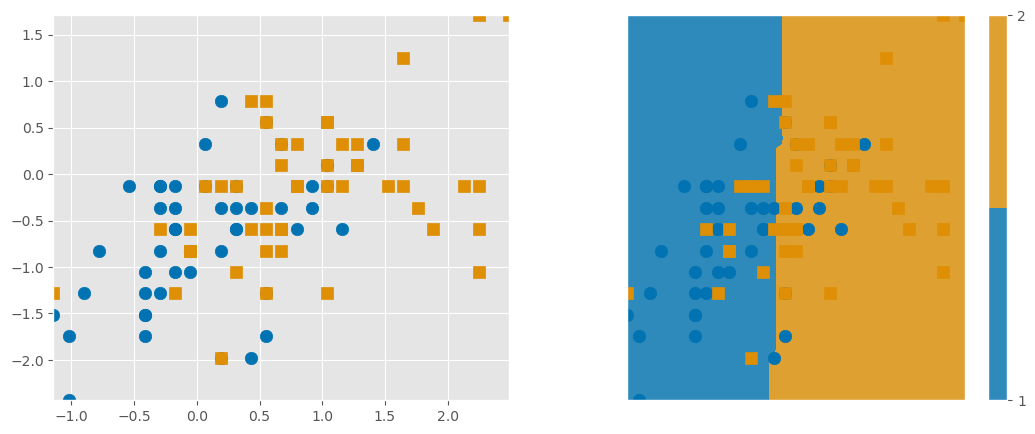
\includegraphics[width=0.9\linewidth]{nuageiris.png}
    \caption{Nuage de points avec frontière de séparation des deux classes}
    \label{fig:placeholder1}
\end{figure}


En utilisant un SVM linéaire pour discriminer les classes versicolor et virginica à partir des deux premières variables de l’iris (longueur et largeur des sépales), nous obtenons une précision d’environ 75 \% sur l’échantillon d’apprentissage et 68 \% sur l’échantillon de test.

On constate que la séparation obtenue n’est pas parfaite : la frontière linéaire coupe au milieu d’une zone où les deux classes se chevauchent, entraînant ainsi de nombreuses erreurs de classification. Ces résultats traduisent le fait que les caractéristiques retenues (longueur et largeur des sépales) ne suffisent pas à distinguer efficacement versicolor et virginica, dont les valeurs de sépales présentent une forte similarité.
    

\subsection{SVM basé sur le noyau polynomial}

Lors de l’utilisation d’un \textit{SVM} avec noyau polynomial, nous obtenons les hyperparamètres suivants : C = 0.0316, \text{degré} = 1 et \gamma = 10.

Les performances obtenues sont : \text{Score apprentissage} \approx  75\%, \quad 
\text{Score test} \approx 68\%.




\begin{figure}[H]
    \centering
    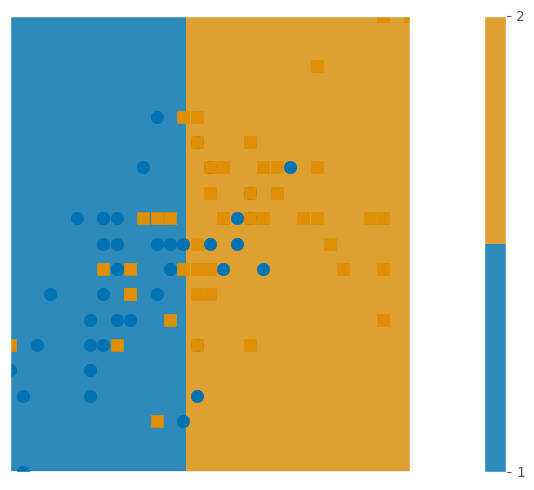
\includegraphics[width=0.45\linewidth]{frontiere.png}
    \caption{Frontière de séparation à l’aide du noyau polynomial}
    \label{fig:placeholder}
\end{figure}


\section{Comparaison SVM linéaire et polynomial}

La comparaison des frontières de décision montre que les noyaux linéaire et polynomial produisent une séparation quasiment identique entre les classes versicolor et virginica. Cela est dû au fait que le degré optimal du noyau polynomial est $1$, ce qui correspond en réalité à un classifieur linéaire. Ainsi, l’ajout d’un noyau polynomial n’apporte aucune amélioration dans ce contexte, car les deux premières variables (sépales) ne permettent pas de bien discriminer les deux classes.

\section{Variation du paramètre C et performances du SVM linéaire}

Voici la représentation graphique d’un jeu de données déséquilibré (90/10) ainsi que les frontières de décision obtenues avec un SVM linéaire pour $C = 1$ et $C = 10^{-3}$.

\begin{figure}[H]
    \centering
    \begin{minipage}{0.47\linewidth}
        \centering
        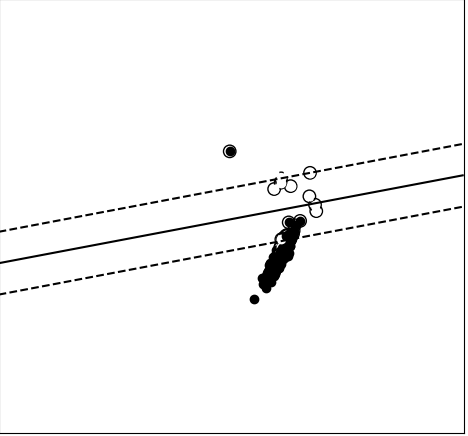
\includegraphics[width=\linewidth]{1.PNG}
        \caption*{C=1}
    \end{minipage}\hfill
    \begin{minipage}{0.47\linewidth}
        \centering
        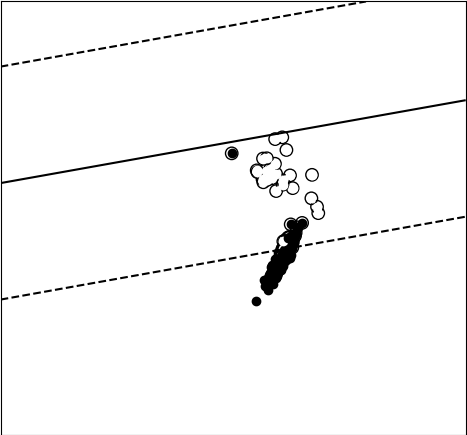
\includegraphics[width=\linewidth]{2.PNG}
        \caption*{C=0.001}
    \end{minipage}\hfill
    \caption{Impact du choix de noyau et le paramètre}
    \label{fig:trois_images}
\end{figure}

On observe que le paramètre $C$ d’un SVM règle le compromis entre la complexité du modèle et la tolérance aux erreurs. 
Lorsque $C$ augmente, l’algorithme cherche à bien séparer toutes les données, ce qui peut donner une frontière compliquée et peu généralisable. 
Lorsque $C$ diminue, le modèle accepte plus d’erreurs et construit une frontière plus simple avec une marge plus large. 

Dans un jeu de données déséquilibré, diminuer $C$ favorise la classe majoritaire (90~\%) au détriment de la classe minoritaire (10~\%). 
La frontière se déplace vers la minorité, qui est alors souvent mal prédite. 
La précision globale peut sembler correcte (environ 90~\%), mais elle est trompeuse car elle reflète surtout la bonne classification de la majorité, tandis que la minorité est mal reconnue.




\section{Analyse de la régularisation avec le paramètre C}
\begin{figure}[H]
    \centering
    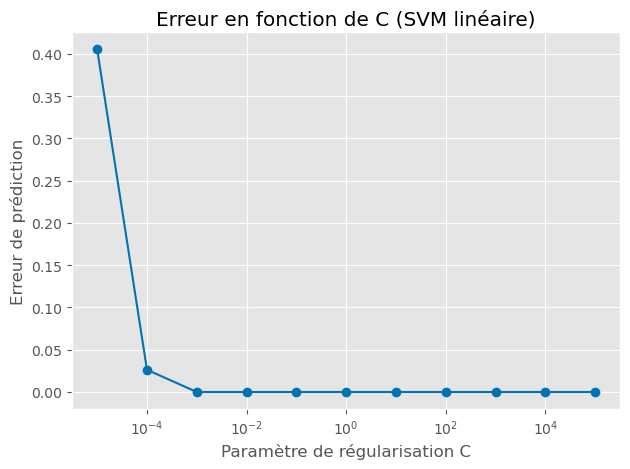
\includegraphics[width=0.75\linewidth]{output.png}
    \caption{Erreur de prédiction en fonction du paramètre C}
    \label{fig:placeholder}
\end{figure}


On observe qu’avec une valeur très faible de $C$ (par exemple $10^{-5}$), l’erreur de prédiction est élevée, autour de 0.40. Cela signifie que la régularisation est trop forte : le modèle accepte trop d’erreurs et sous-apprend (underfitting).

Dès que $C$ augmente (à partir de $10^{-4}$), l’erreur chute brutalement et devient quasi nulle. Pour $C \geq 10^{-3}$, l’erreur reste à 0, ce qui montre que le modèle parvient à classer parfaitement les données d’apprentissage.

\section{Dégradation des performances avec des variables non pertinentes}

\begin{table}[H]
\centering
\begin{tabular}{|c|c|c|}
\hline
\textbf{Nb. de variables de nuisance} & \textbf{Score test sans nuisance} & \textbf{Score test avec nuisance} \\ \hline
0   & 0.916 & 0.563 \\ \hline
10  & 0.900 & 0.511 \\ \hline
20  & 0.863 & 0.500 \\ \hline
50  & 0.953 & 0.505 \\ \hline
100 & 0.921 & 0.500 \\ \hline
\end{tabular}
\caption{Scores de test avec et sans variables de nuisance pour un SVM linéaire.}
\label{tab:svm_nuisance}
\end{table}

On observe que, sans variables de nuisance, le score de test reste élevé (entre 86\% et 95\%). 
En revanche, dès que des variables de bruit sont ajoutées, la performance chute fortement et se stabilise autour de 50\%. 
Cela montre que l’introduction de caractéristiques non informatives perturbe l’apprentissage du SVM 
et dégrade sa capacité à bien généraliser sur de nouvelles données.


\section{Amélioration de la généralisation par PCA }

\begin{table}[H]
\centering

\begin{tabular}{|c|c|c|}
\hline
\textbf{Nombre de composantes} & \textbf{Score apprentissage} & \textbf{Score test} \\
\hline
5  & 0.626 & 0.616 \\ \hline
10 & 0.642 & 0.600 \\ \hline
20 & 0.611 & 0.632 \\ \hline
30 & 0.711 & 0.563 \\
\hline
\end{tabular}
\label{tab:pca_svm}
\caption{Résultats de la PCA avec \texttt{whiten=True} pour accélérer et stabiliser l’échelle des composantes}
\end{table}



Les résultats obtenus montrent que le choix du nombre de composantes principales a un impact direct sur la performance du SVM linéaire : avec 10 composantes, le modèle atteint des scores équilibrés entre apprentissage (0,64) et test (0,60), tandis qu’avec 20 composantes, il généralise légèrement mieux (0,61 en apprentissage et 0,63 en test). En revanche, lorsque le nombre de composantes est porté à 30, la précision d’apprentissage augmente (0,71) mais celle du test chute fortement (0,56), signe d’un surapprentissage.

Ainsi, la réduction de dimension par PCA illustre bien le compromis biais/variance : trop peu de composantes entraînent une perte d’information, tandis qu’un excès de dimensions réintroduit du bruit et dégrade la généralisation. Dans ce cas précis, un choix autour de 20 composantes semble offrir le meilleur équilibre.

\section{Biais introduit lors du prétraitement des données}

Le biais vient du fait qu'on standardise les donnéees sur l'ensemble complet(train/test) avant la separation, ce qui introduit une fuite d'information surestime la performances.

\newpage

\end{document}
